\documentclass[slovak]{beamer}
\usepackage{appendixnumberbeamer}
\usepackage[utf8]{inputenc}
\usepackage[T1]{fontenc}
\usepackage{graphicx}

\usepackage[slovak]{babel}

\usetheme{Boadilla}

\title[$L(2,1)$-farbenia grafov]{Farbenia grafov s obmedzeniami do vzdialenosti dva}
\author[Bc. Jaroslav Petrucha]{Bc. Jaroslav Petrucha \\ školiteľ: RNDr. Michal Forišek, PhD.}
\date{14. 6. 2018}


\deftranslation[to=Slovak]{Theorem}{Veta}

\begin{document}

\begin{frame}
\titlepage
\end{frame}

\begin{frame}{$L(2,1)$-farbenie}
    \begin{itemize}
        \item Ohodnotenie vrcholov prirodzenými číslami
        \begin{itemize}
            \item Susedné vrcholy majú veľký rozdiel
            \item Vrcholy so spoločným susedom sa líšia
        \end{itemize}
    \end{itemize}
    \begin{center}
        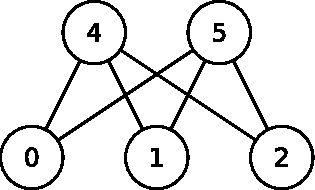
\includegraphics[width=0.3\textwidth]{grafy/l21-example.pdf}
    \end{center}
\end{frame}

\begin{frame}{Súvisiace problémy}
    \begin{itemize}
        \item Skúmame rozsah priradených hodnôt
        \item Rozhodovacie aj optimalizačné problémy
        \begin{itemize}
            \item Stačí rozsah $k$?
            \item Aký je minimálny rozsah?
        \end{itemize}
        \item{$\mathcal{NP}$-ťažký na mnohých triedach}
        \begin{itemize}
            \item Planárne grafy
            \item Čiastočné $2$-stromy, bipartitné grafy
        \end{itemize}
    \end{itemize}
\end{frame}

\begin{frame}{Polynomiálny algoritmus}
    \begin{itemize}
        \item Špeciálne triedy grafov
        \begin{itemize}
            \item Stromy, cyklové stromy
            \item Vonkajšoplanárne grafy
        \end{itemize}
        \item Lokálne riešenie malých podproblémov
    \end{itemize}
\end{frame}

\begin{frame}{Všeobecný algoritmus}
    \begin{itemize}
        \item Dynamické programovanie
        \begin{itemize}
            \item FIXME: Časová zložitosť
            \item FIXME: Havet et al.
        \end{itemize}
        \item Množiny všetkých čiastočných farbení
        \begin{itemize}
            \item $O^*(2.6488^n)$
            \item FIXME: Junosza-Szaniawski et al.
        \end{itemize}
    \end{itemize}
\end{frame}

\begin{frame}{Vlastná práca - mosty}
    \begin{itemize}
        \item Mostová hrana $e = \{u,v\}$
        \item Vrcholy v rôznych komponentoch sú ďaleko
        \item Ofarbíme $u$ a $v$, komponenty riešime zvlášť
    \end{itemize}
    \begin{center}
        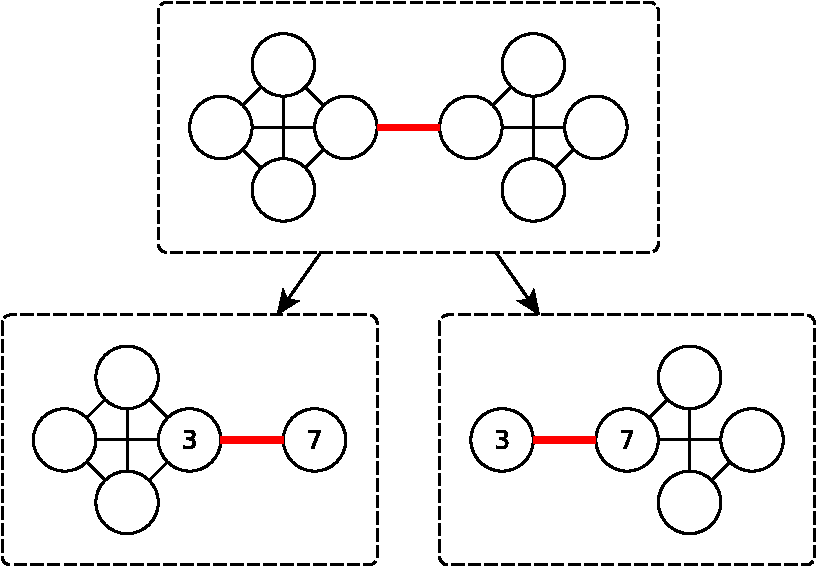
\includegraphics[width=0.5\textwidth]{grafy/bridgesplit.pdf}
    \end{center}
\end{frame}

\begin{frame}{Pozorovania}
    \begin{itemize}
        \item Musíme riešiť rozhodovací problém
        \begin{itemize}
            \item Máme daný rozsah $k$
        \end{itemize}
        \item Najlepšie je rovnomerné rozdelenie
        \begin{itemize}
            \item Za malý komponent platíme viac, než ušetríme
        \end{itemize}
        \item Ak je komponent príliš malý, môžeme ho ignorovať
        \begin{itemize}
            \item Vzhľadom na rozsah $k$
            \item Zaručene sa dá dofarbiť
        \end{itemize}
    \end{itemize}
\end{frame}

\begin{frame}{Orezanie malého komponentu}
    \begin{center}
        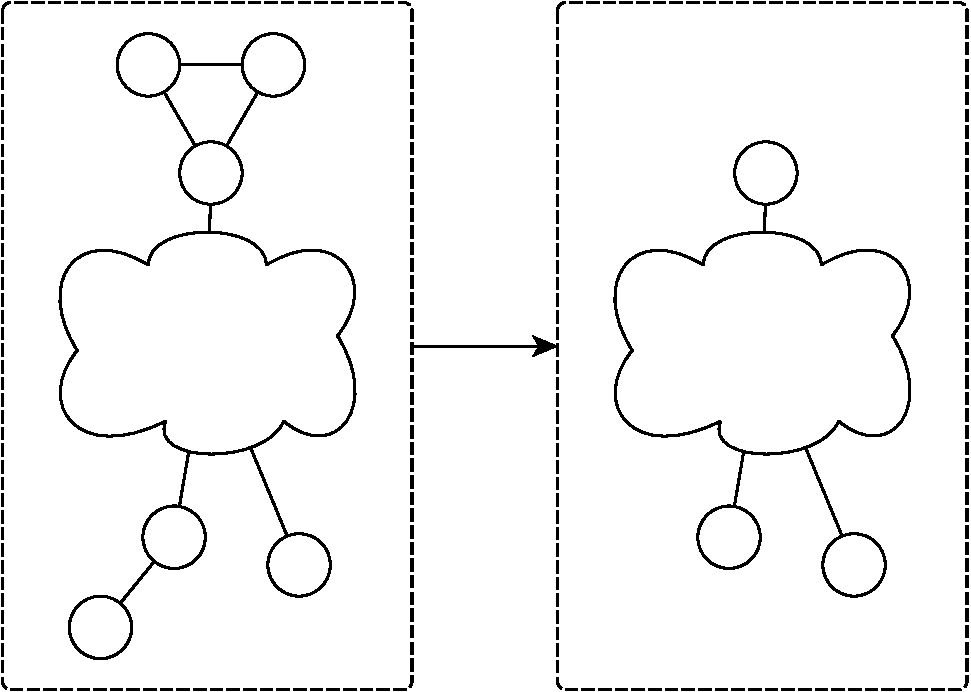
\includegraphics[width=0.6\textwidth]{grafy/zanedbaj.pdf}
    \end{center}
\end{frame}

\begin{frame}{Základná myšlienka}
    \begin{itemize}
        \item Pre rozsah $k \leq 5$ použijeme iný algoritmus
        \item Odstránime malé komponenty
        \item Nájdeme stredný komponent $K_s$
        \item Ofarbíme všetky mosty v $K_s$
        \item Pre každú možnosť vyriešime menší problém
    \end{itemize}
\end{frame}

\begin{frame}{Výsledok}
    \begin{itemize}
        \item Stačí riešiť grafy bez netriviálnych mostov
    \end{itemize}
    \begin{center}
        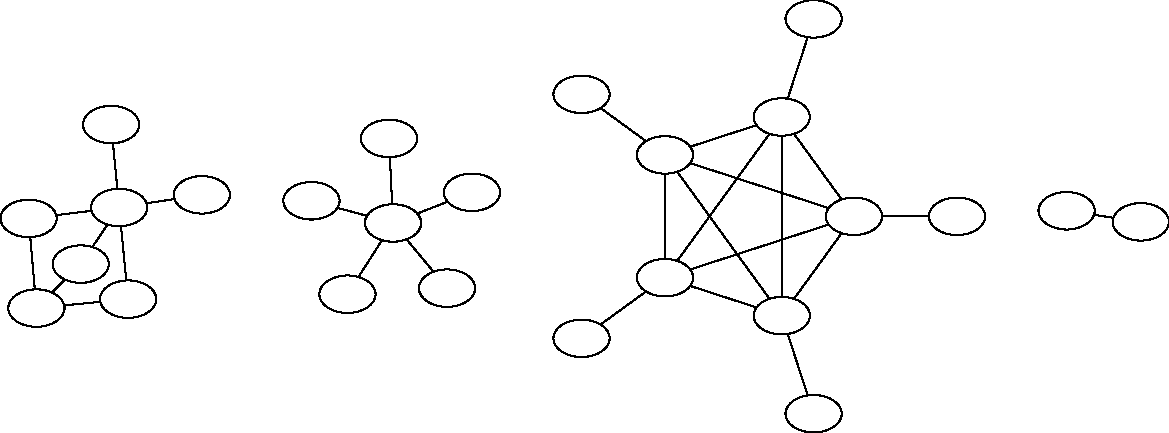
\includegraphics[width=0.7\textwidth]{grafy/ec2-example.pdf}
    \end{center}
    \begin{itemize}
        \item Zo špecifického $O^*(\alpha^n)$ dostaneme rovnako
        rýchle všeobecné riešenie
        \item Pre $6 \leq k \leq 11$ horšia časová zložitosť
        \begin{itemize}
            \item Na niektorých zlých typoch grafov
        \end{itemize}
    \end{itemize}
\end{frame}

\begin{frame}{Algoritmus Junosza-Szaniawski}
    \begin{itemize}
        \item Každý graf má triviálne $(2n)$-farbenie
        \item Postupne počítame tabuľky $T_0, T_1 \ldots T_{2n}$
        \item $T_k$ popisuje všetky čiastočné farbenia s rozsahom $k$
        \item Hlavná časť algoritmu je počítanie $\oplus: T_k \mapsto T_{k+1}$
    \end{itemize}
\end{frame}

\begin{frame}{Algoritmus Junosza-Szaniawski}
    \begin{itemize}
        \item $T_k$ popisuje čiastočné farbenia s rozsahom $k$
        \item Stačí vedieť, ktoré vrcholy majú farbu $k$ a ktoré sú ofarbené
        \item Stavy sa nazývajú \emph{vlastné páry}
        \item Počet vlastných párov aj časová zložitosť je $O^*(2.6488^n)$
        \item Najviac vlastných párov majú stromy
    \end{itemize}
\end{frame}

\begin{frame}{Vlastná práca - planárne grafy}
    \begin{theorem}[Lipton, Tarjan]
        Nech $G$ je ľubovoľný $n$-vrcholový planárny graf. Vrcholy $G$ sa dajú rozdeliť
        do množín $A, B, C$ tak, že neexistuje hrana medzi vrcholom v $A$ a vrcholom v $B$,
        veľkosť množiny $A$ aj množiny $B$ je nanajvýš $\frac{n}{2}$ a veľkosť množiny $C$ je nanajvýš
        $\frac{2\sqrt{2}}{1 - \sqrt{2/3}} \sqrt{n}$.
    \end{theorem}
\end{frame}

\begin{frame}{Základná myšlienka}
    \begin{itemize}
        \item Nájdeme vrcholový separátor $S$ s $O(\sqrt{n})$ vrcholmi
        \item Čiastočné farbenia rozdelíme podľa ofarbenia $S$ a okolia
        \item Pre komponenty $G - S$ počítame množiny $T_i$ nezávisle
    \end{itemize}
\end{frame}

\begin{frame}{Ukážka na príklade}
    FIXME: Obrázok
\end{frame}

\begin{frame}{Riešenie pre planárne grafy}
    \begin{itemize}
        \item Mierne odlišné riešenie podľa veľkosti okolia separátora $S$
        \item Časová zložitosť v oboch prípadoch $O^*(2.2^{n + o(n)})$
        \item Funguje pre grafy s $O(n^{1 - \varepsilon})$ separátorom
    \end{itemize}
\end{frame}

\begin{frame}{Vyvážene rozdeliteľné grafy}
    \begin{itemize}
        \item Vrcholy vieme rozdeliť do množín $A$ a $B$
        \item $A$ aj $B$ majú nanajvýš $\frac{2n}{3}$ vrcholov
        \item Počet vrcholov so susedom v druhej množine je nanajvýš $\frac{n}{4}$
        \item Časová zložitosť algoritmu je $O^*(2.614^n)$
    \end{itemize}

    %FIXME: obrázok
\end{frame}

\begin{frame}{Vlastné páry na $2$-hranovo súvislých grafoch}
    \begin{itemize}
        \item Vyplýva z práce k mostom
        \item Generujeme minimálne $2$-hranovo súvislé grafy
        \item Z grafov s nanajvýš $20$ vrcholmi má najviac kružnica
        \item Kružnica s $n$ vrcholmi má $O(2.5943^n)$ vlastných párov
    \end{itemize}
\end{frame}

\begin{frame}{Generovanie grafov}
    \begin{center}
        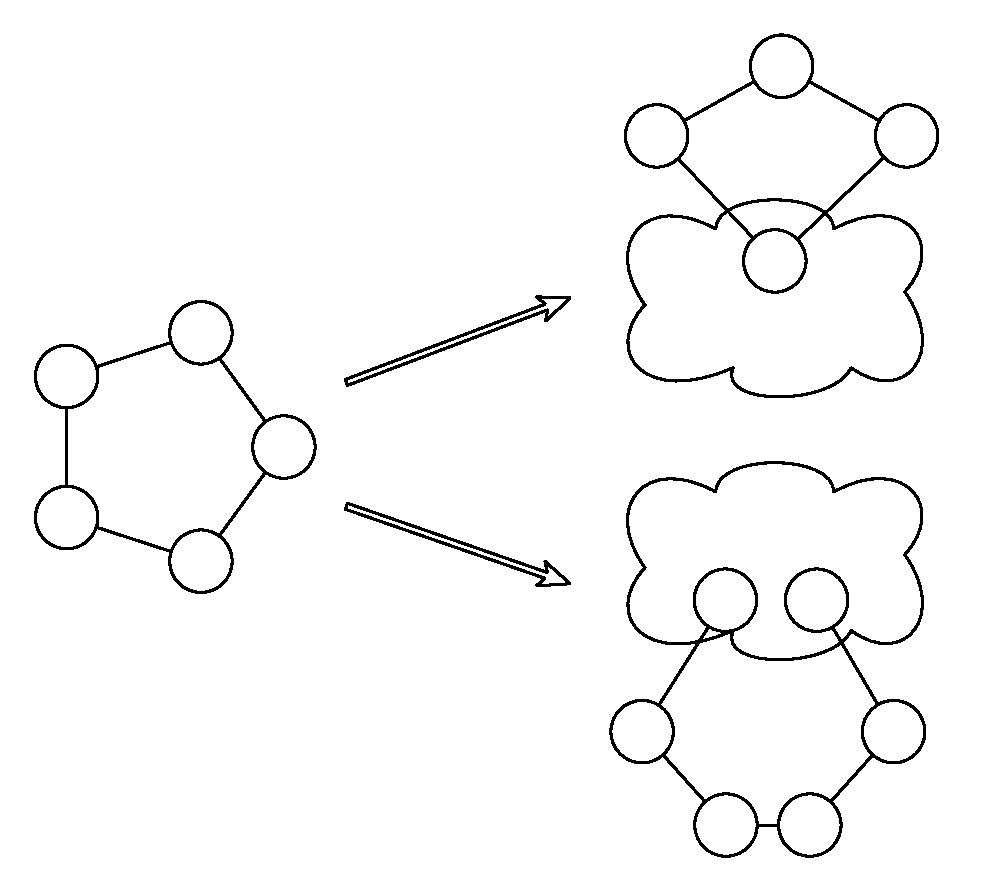
\includegraphics[width=0.6\textwidth]{grafy/gengraph.pdf}
    \end{center}
\end{frame}

\begin{frame}{Záver}
    \begin{itemize}
        \item Zjednodušenie problému na chlpaté $2$-hranovo súvislé grafy
        \item Rýchlejší algoritmus pre planárne grafy
        \item Rýchlejší algoritmus pre vyvážene rozdeliteľné grafy
        \item Generátor minimálne $2$-hranovo súvislých grafov
        \item Experiment nad $2$-hranovo súvislými grafmi
    \end{itemize}
\end{frame}

\begin{frame}[plain,c]

\begin{center}
\Huge Ďakujem za pozornosť!
\end{center}

\end{frame}

\appendix

\begin{frame}
1
\end{frame}

\begin{frame}
2
\end{frame}
\end{document}
